\documentclass{report}

\input{~/latex/template/preamble.tex}
\input{~/latex/template/macros.tex}

\title{\Huge{Graph and Tree Theory Notes}}
\author{\huge{Matt Warner}}
\date{\huge{}}
\pagestyle{fancy}
\fancyhf{}
\rhead{GRAPH AND TREE THEORY}
\lhead{\leftmark}
\cfoot{\thepage}
% \usepackage[default]{sourcecodepro}
% \usepackage[T1]{fontenc}
% \definecolor{doc}{R

\pgfpagesdeclarelayout{boxed}
{
  \edef\pgfpageoptionborder{0pt}
}
{
  \pgfpagesphysicalpageoptions
  {%
    logical pages=1,%
  }
  \pgfpageslogicalpageoptions{1}
  {
    border code=\pgfsetlinewidth{1.5pt}\pgfstroke,%
    border shrink=\pgfpageoptionborder,%
    resized width=.95\pgfphysicalwidth,%
    resized height=.95\pgfphysicalheight,%
    center=\pgfpoint{.5\pgfphysicalwidth}{.5\pgfphysicalheight}%
  }%
}

\pgfpagesuselayout{boxed}





\begin{document}
	\maketitle
	\tableofcontents
	\pagebreak
\begin{LARGE}
		\textbf{\section{Trails, Paths, and Circuits}}
\end{LARGE}

\thmcon{
	\textbf{\underline{Definition}}
	\vspace{3mm}

Let $G$ be a graph, and let $v$ and $w$ be vertices in $G$.
\vspace{3mm}

A walk from $v$ to $w$ is a finite alternating sequence of adjacent vertices and edges of $G$. Thus a walk has the form

$$
v_0 e_1 v_1 e_2 \cdots v_{n-1} e_n v_n
$$

where the $v$ 's represent vertices, the $e$ 's represent edges, $v_0=v, v_n=w$, and for each $i=1,2, \ldots n, v_{i-1}$ and $v_i$ are the endpoints of $e_i$. The trivial walk from $v$ to $v$ consists of the single vertex $v$.
\vspace{3mm}
\begin{itemize}
  
\item A trail from $v$ to $w$ is a walk from $v$ to $w$ that does not contain a repeated edge.
\item A path from $v$ to $w$ is a trail that does not contain a repeated vertex.

\item A closed walk is a walk that starts and ends at the same vertex.

\item A circuit is a closed walk that contains at least one edge and does not contain a repeated edge.

\item A simple circuit is a circuit that does not have any other repeated vertex except the first and last.
\end{itemize}
}
\bigbreak \noindent 
\begin{center}
  \begin{table}[h]
    \centering
    \begin{tabular}{|l|c|c|c|c|}
        \hline
        & \textbf{Repeated} & \textbf{Repeated} & \textbf{Starts and Ends} & \textbf{Must Contain} \\
        & \textbf{Edge?} & \textbf{Vertex?} & \textbf{at Same Point?} & \textbf{at Least One Edge?} \\
        \hline
        Walk & allowed & allowed & allowed & no \\
        \hline
        Trail & no & allowed & allowed & no \\
        \hline
        Path & no & no & no & no \\
        \hline
        Closed Walk & allowed & allowed & yes & no \\
        \hline
        Circuit & no & allowed & yes & yes \\
        \hline
        Simple Circuit & no & \begin{tabular}{@{}c@{}}first and\\last only\end{tabular} & yes & yes \\
        \hline
    \end{tabular}
\end{table}
\end{center}
\bigbreak \noindent 
\ex{}{Determine which of the following walks are trails, paths, circuits, or simple circuits.

\begin{enumerate}
	\begin{multicols}{2}
	\item $v_1,e_1,v_2,e_3,v_3,e_4,v_3,e_5,v_4$
	\item $e_1,e_3,e_5,e_5,e_6$
	\end{multicols}
	\begin{multicols}{2}
	\item $v_2 v_3 v_4 v_5 v_3 v_6 v_2$
		\item $v_1e_1v_2e_1v_1$
	\end{multicols}
	\begin{multicols}{2}
		\item $v_2,v_3,v_4,v_5,v_6,v_2$
		\item $v_1$
		\end{multicols}
\end{enumerate}
}
\begin{figure}[ht]
	\centering
	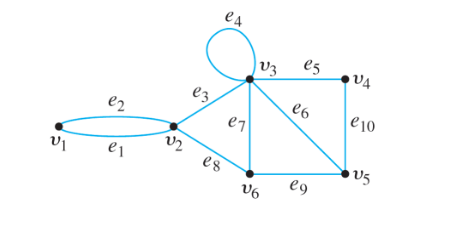
\includegraphics[width=0.5\textwidth]{figure1.png}
\end{figure}
\newpage

\pf{Soultion}

1. this walk is a Trail, since it does not contain any repeted edges.
\vspace{2mm}

2. This is just a walk and nothing else.
\vspace{2mm}

3. This walk is a Closed walk and is also a circuit, but not a simple circuit.
\vspace{2mm}

4. This is just a closed walk, it cant be a circuit since there is a repeated edge.
\vspace{2mm}

5. This is a closed walk, as well as a simple circuit.
\vspace{2mm}

6. This is a closed walk, as well as a trail, not a circuit becuase the walk does not contain any edges.
\bigbreak \noindent \bigbreak \noindent
\begin{LARGE}
	\textbf{\section{Subgraphs}}
\end{LARGE}
\bigbreak \noindent
\thmcon{
	\textbf{\underline{Definition}}
	\vspace{3mm}
	
A graph $H$ is said to be a subgraph of a graph $G$ if, and only if, every vertex in $H$ is also a vertex in $G$, every edge in $H$ is also an edge in $G$, and every edge in $H$ has the same endpoints as it has in $G$.

}
\bigbreak \noindent \bigbreak \noindent
\ex{}{
	List all subgraphs of the graph $G$ with vertex set $\{v_1,v_2\}$ and edge set $\{e_1,e_2,e_3\}$, where the endpoints of $e_1$ are $v_1$ and $v_2$, the endpoints of $e_2$ are $v_1$ and $v_2$, and $e_3$ is a loop at $v_1$.
	\vspace{3mm}

	$G$ can be drawn as shown below.
	\vspace{2mm}


}

\begin{figure}[ht]
\centering
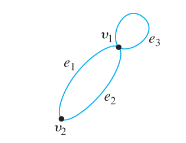
\includegraphics[width=0.3\textwidth]{ figure2.png }
\caption{$G$}
\end{figure}
\newpage

\noindent There are 11 subgraphs of $G$, which can be grouped according to those that do not have any edges, those that have one edge, those that have two edges, and those that have three edges.

\begin{figure}[ht]
\centering
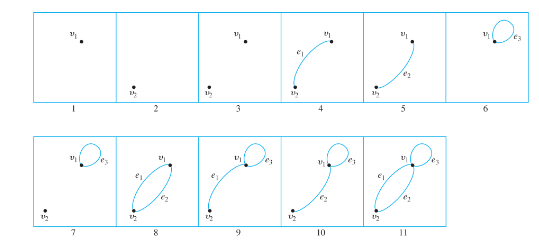
\includegraphics[width=0.5\textwidth]{ figure3.png }
\caption{Subgraphs of $G$}
\end{figure}
\bigbreak \noindent \bigbreak \noindent
\begin{LARGE}
	\textbf{\section{Connectedness}}
\end{LARGE}
\bigbreak \noindent
\thmcon{
	\textbf{\underline{Definition}}
	\vspace{3mm}
	
	Let $G$ be a graph. Two \textbf{vertices, $v$ and $w$ of $G$ are connected} if, and only if, there is a walk from $v$ to $w$. 
	\vspace{2mm}
	
	The \textbf{graph $G$ is connected} if, and only if, given \textit{any} two vertices $v$ and $w$ in $G$, there is a walk from $v$ to $w$. Symbolically:
	\vspace{3mm}
	
	{\centerline{$G$ is connected $\longleftrightarrow$ $\forall$ vertices $v$ and $w$ in $G, \exists$ a walk from $v$ to $w$. }}
}
\bigbreak \noindent
\nt{
If you take the negation of this definition, you will see that a graph $G$ is \textit{not connected} if, and only if, there exists two vertices of $G$ that are not connected by any walk.}
\bigbreak \noindent \bigbreak \noindent
\ex{}{
	Which of the following graphs are connected?
	\vspace{3mm}

	The graphs are listed below
}
\begin{figure}[ht]
\centering
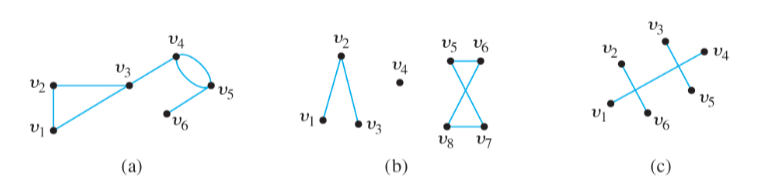
\includegraphics[width=0.8\textwidth]{ figure4.png }
\end{figure}

\pf{Solution}

Graph $A$ is connected \hspace{14mm} Graph $B$ is not connected \hspace{14mm} Graph $C$ is also not connected
\newpage

\begin{large}
 Some useful facts relating circuits and connectedness are collected in the following lenma. 
\end{large}
\bigbreak \noindent
\mlenma{}{
Let $G$ be a graph.
\vspace{2mm}

a. If $G$ is connected, then any two distinct vertices of $G$ can be connected by a path.
\vspace{2mm}

b. If vertices $v$ and $w$ are part of a circuit in $G$ and one edge is removed from the circuit, then there still exists a trail from $v$ to $w$ in $G$.
\vspace{2mm}

c. If $G$ is connected and $G$ contains a circuit, then an edge of the circuit can be removed without disconnecting $G$.
}
\bigbreak \noindent \bigbreak \noindent
\ex{}{
	Find all connected components of the following graph $G$.
}
\begin{figure}[ht]
\centering
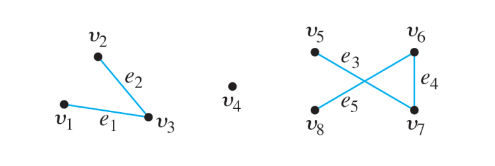
\includegraphics[width=0.7\textwidth]{ figure5.png }
\end{figure}
\pf{Solution}

\noindent $G$ has three connected components: $H_1,H_2$ and $H_3$ with vertex sets $V_1,V_2$, and $V_3$ and edge sets $E_1,E_2$, and $E_3$

\begin{center}
$$\begin{array}{ll}
V_1=\left\{v_1, v_2, v_3\right\}, & E_1=\left\{e_1, e_2\right\}, \\
V_2=\left\{v_4\right\}, & E_2=\varnothing, \\
V_3=\left\{v_5, v_6, v_7, v_8\right\}, & E_3=\left\{e_3, e_4, e_5\right\} .
\end{array}$$
\end{center}
\bigbreak \noindent \bigbreak \noindent 
\begin{LARGE}
	\textbf{\section{Euler Circuits}}
\end{LARGE}
\thmcon{
	\textbf{\underline{Definition}}
	\vspace{3mm}

	Let $G$ be a graph. An Euler circuit for $G$ is a circuit that contains every vertex and every edge of $G$. That is, an Euler circuit for $G$ is a sequence of adjacent vertices and edges in $G$ that has at least one edge, starts and ends at the same vertex, uses every vertex of $G$ at least once, and uses every edge of $G$ exactly once.
}
\bigbreak \noindent
\thm{}{If a graph has a Euler circuit, then every vertex of the graph has positive even degree.
	\vspace{1mm}

	If some vertex of a graph has odd degree, then the graph does not have a Euler circuit
}
\newpage
\ex{}{
	\vspace{2mm}

	Show that the graph below does not have a Euler circuit.
}
\begin{figure}[ht]
\centering
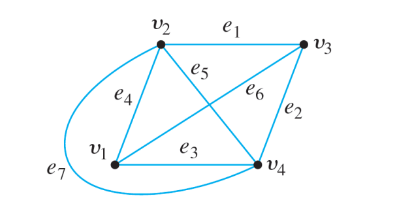
\includegraphics[width=0.5\textwidth]{ figure6.png }
\end{figure}

\pf{Solution}

\vspace{2mm}

	The vertices $v_1,$ and $v_3$ both have odd degrees (degree 3). So the graph cannot be a Euler circuit.
\bigbreak \noindent \bigbreak \noindent
\nt{
If a graph $G$ is connected and the degree of every vertex of $G$ is a postive even integer, then $G$ has a Euler circuit.
}
\bigbreak \noindent
\begin{large}
	\textbf{\subsection{Euler Trails}} 
\end{large}
\bigbreak \noindent 
\thmcon{
	\textbf{\underline{Definition}}
	\vspace{3mm}

	Let $G$ be a graph, and let $v$ and $w$ be two distinct vertices of $G$. An Euler trail from $v$ to $w$ is a sequence of adjacent edges and vertices that starts at $v$, ends at $w$, passes through every vertex of $G$ at least once, and traverses every edge of $G$ exactly once.
}
\bigbreak \noindent 

\cor{}{Let $G$ be a graph, and let $v$ and $w$ be two distinct vertices of $G$. There is an Euler trail from $v$ to $w$ if, and only if, $G$ is connected, $v$ and $w$ have odd degree, and all other vertices of $G$ have positive even degree.}
\bigbreak \noindent \bigbreak \noindent \bigbreak \noindent 
\ex{}{
	The floor plan shown below is for a house that is open for public viewing. Is it possible to find a trail that starts in room $A$, ends in room $B$, and passes through every interior doorway of the house exactly once? If so, find such a trail.
}
\newpage
\begin{figure}[ht]
\centering
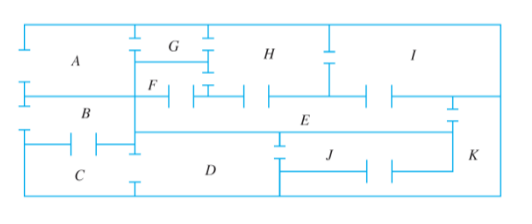
\includegraphics[width=0.5\textwidth]{ figure7.png }
\end{figure}

{\centerline{We can represent this floor plan as a graph:}}
\begin{figure}[ht]
\centering
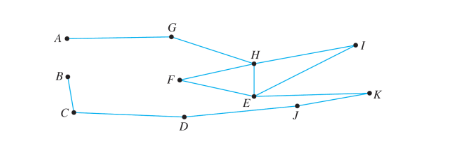
\includegraphics[width=0.5\textwidth]{figure8.png }
\end{figure}

Each vertex of this graph has an even degree except for $A$ and $B$, hence by Corollary 0.4.1 \\ \indent there is an Euler trail from $A$ to $B$ one such trail is

$$ A - G - H - F - E - I - H - E - K - J - D - C - B$$
\bigbreak \noindent \bigbreak \noindent 
\begin{LARGE}
	\textbf{\section{Hamiltonian Circuits}}
\end{LARGE}
\bigbreak \noindent
\thmcon{
	\textbf{\underline{Definition}}
	\vspace{3mm}

	Given a graph $G$, a \textbf{Hamiltonian circuit} for $G$ is a simple circuit that includes every vertex of $G$. That is, a Hamiltonian circuit for $G$ is a sequence of adjacent vertices and distinct edges in which every vertex of $G$ appears exactly once, except for the first and the last, which are the same.
}
\bigbreak \noindent

\mprop{}{If a graph $G$ has a Hamiltonian circuit, then $G$ has a subgraph $H$ with the following properties:
	\vspace{2mm}	  

1. $H$ contains every vertex of $G$.
\vspace{2mm}

2. $H$ is connected.
\vspace{2mm}

3. $H$ has the same number of edges as vertices.
\vspace{2mm}

4. Every vertex of $H$ has degree 2 .}
\bigbreak \noindent \bigbreak \noindent
\newpage
\begin{large}
	\textbf{\section{Matrices}} 
\end{large}
\thmcon{
	\textbf{\underline{Definition}}
	\vspace{3mm}

	Matrices are two-dimensional analogues of sequences.
	\vspace{2mm}

	They also are called two-dimensional arrays
	\vspace{4mm}

An $m \times n$ (read " $m$ by $n$ ") matrix A over a set $S$ is a rectangular array of elements of $S$ arranged into $m$ rows and $n$ columns:
\vspace{5mm}

	$\mathbf{A}=\left[\begin{array}{cccccc}
a_{11} & a_{12} & \cdots & a_{1 j} & \cdots & a_{1 n} \\
a_{21} & a_{22} & \cdots & a_{2 j} & \cdots & a_{2 n} \\
\vdots & \vdots & & \vdots & & \vdots \\
a_{i 1} & a_{i 2} & \cdots & a_{i j} & \cdots & a_{i n} \\
\vdots & \vdots & & \vdots & & \vdots \\
a_{m 1} & a_{m 2} & \cdots & a_{m j} & \cdots & a_{m n}
\end{array}\right] \leftarrow \text { ith row of } \mathrm{A}$
\vspace{5mm}

We write \textbf{A} = $(a_{ij})$
\vspace{5mm}

The $i$th row of A is 
$$
\left[\begin{array}{llll}
a_{i 1} & a_{i 2} & \ldots & a_{i n}
\end{array}\right]
$$
\vspace{3mm}

and the $j$th column of A is 
$$
\left[\begin{array}{c}
a_{1 j} \\
a_{2 j} \\
\vdots \\
a_{m j}
\end{array}\right]
$$
\vspace{6mm}

A matrix for which the numbers of row and columns are equal is called a \textbf{square matrix}
\vspace{5mm}

If $\mathbf{A}$ is a square matrix of size $n \times n$, then the main diagonal of $\mathbf{A}$ consists of all the entries $a_{11}, a_{22}, \ldots, a_{n n}$
}
\bigbreak \noindent
\begin{figure}[ht]
\centering
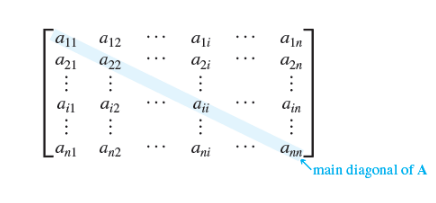
\includegraphics[width=0.55\textwidth]{ figure9.png }
\captionsetup{justification=centering,margin={-1cm,0cm}}
\caption{Square matrix diagonal}
\end{figure}
\newpage
\ex{}{
	The following is a 3 x 3 matrix over the set of integers.
	\vspace{3mm}

\begin{center}
	$\mathbf{A}=\left[\begin{array}{rrr}
	1 & 0 & -3 \\
	4 & -1 & 5 \\
	-2 & 2 & 0
\end{array}\right]$ 
\end{center}
\vspace{3mm}
\begin{enumerate}
	\item What is $a_{23}$, the entry in row 2 , column 3 ?
	\item What is the second column of $\boldsymbol{A}$ ?
	\item What are the entries in the main diagonal of $\mathbf{A}$ ?
\end{enumerate}
}
\pf{Solution}

\begin{large}
\begin{enumerate}
  
	\item $a_{23} = 5$
		\vspace{2mm}

	\item $\left[\begin{array}{r}
		0 \\
		-1 \\
		2
		\end{array}\right]$
		\vspace{2mm}

	\item $1, -1, 0$

\end{enumerate}  
\end{large}
\bigbreak \noindent \bigbreak \noindent
\begin{large}
	\textbf{\subsection{Matrices and Directed Graphs}}
\end{large}
\bigbreak \noindent
  
\begin{figure}[ht]
\centering
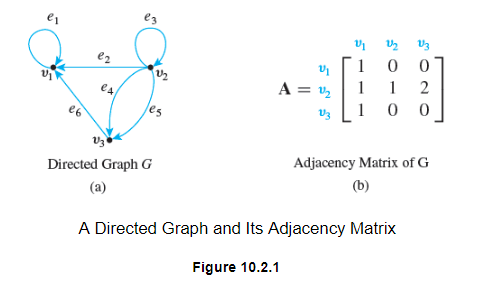
\includegraphics[width=0.5\textwidth]{ figure10.png }
\end{figure}
\bigbreak \noindent
\nt{As shown by the figure above, the adjacency matrix holds holds all the data for the directed graph, each entry in the matrix is either a $1$ or $0$, the entry is a 0 if the two vertices are not adjacent, and a 1 if they are adjacent, with the number increasing by the amount of edges that connect the vertices.}
\newpage
\ex{}{
	The two graphs show below are identical and differ only in the ordering of their vertices.
	\vspace{4mm}

	Find their adjacency matrices
}
\begin{figure}[ht]
\centering
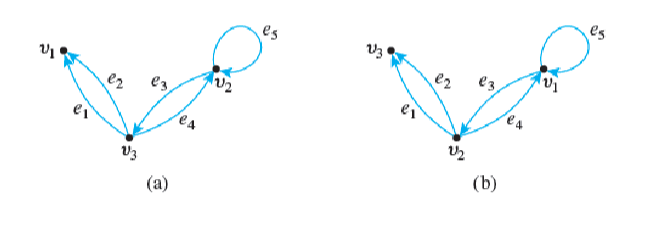
\includegraphics[width=0.7\textwidth]{ figure11.png }
\end{figure}

\pf{Solution}

\[
A = 
\begin{bmatrix}
0 & 0 & 0 \\
0 & 1 & 1 \\ 
2 & 1 & 0
\end{bmatrix}
\]
\vspace{2mm}

\[
B = 
\begin{bmatrix}
	1 & 1 & 0 \\
	1 & 0 & 2 \\
	0 & 0 & 0 
\end{bmatrix}
\]
\bigbreak \noindent \bigbreak \noindent
\begin{large}
	\textbf{\subsection{Symmetric Matrices}} 
\end{large}
\thmcon{
	\textbf{\underline{Definition}}
	\vspace{3mm}

	An $n \times n$ square matrix $\mathbf{A}=\left(a_{i j}\right)$ is called symmetric if, and only if, for every $i$ and $j=1,2, \ldots, n$,
$$
a_{i j}=a_{j i}
$$
}
\bigbreak \noindent 
\ex{}{
	Which of the following matrices are symmetric?
	\vspace{5mm}

\begin{minipage}{0.3\textwidth}
    \[
    A =
    \begin{bmatrix}
    1 & 0 \\
    1 & 2
    \end{bmatrix}
    \]
\end{minipage}
\begin{minipage}{0.3\textwidth}
    \[
    B =     
    \begin{bmatrix}
    0 & 1 & 2 \\    
    1 & 1 & 0 \\ 
    2 & 0 & 3
    \end{bmatrix}
    \]
\end{minipage}
\begin{minipage}{0.3\textwidth}
    \[
    C = 
    \begin{bmatrix}
    2 & 0 & 0 \\
    0 & 1 & 0
    \end{bmatrix}
    \]
\end{minipage}
}
\pf{Soultion}

Only graph $B$ is symmetric
\vspace{2mm}

In matrix $A$ the entry in the first row and the second column differs from the entry in the second row and 

the first column; the matrix, $C$, is not even square.
\newpage
\begin{large}
	\textbf{\subsection{Matrix Multiplication}} 
\end{large}
\bigbreak \noindent
The product of two matrices is built up of \textit{scalar} or \textit{dot} products of their individual rows and columns.
\bigbreak \noindent
\thmcon{
	\textbf{\underline{Definition}}
	\vspace{3mm}

	Suppose that all entries in matrices $\mathbf{A}$ and $\mathbf{B}$ are real numbers. If the number of element, $n$, in the $i$ th row of $\mathbf{A}$ equals the number of elements in the $j$ th column of $\mathbf{B}$, then the scalar product or dot product of the $i$ th row of $\mathbf{A}$ and $j$ th column of $\mathbf{B}$ is the real number obtained as follows:
$$
\left[\begin{array}{llll}
a_{i 1} & a_{i 2} & \cdots & a_{i n}
\end{array}\right]\left[\begin{array}{c}
b_{1 j} \\
b_{2 j} \\
\vdots \\
b_{n j}
\end{array}\right]=a_{i 1} b_{1 j}+a_{i 2} b_{2 j}+\cdots+a_{i n} b_{n j}
$$
\bigbreak \noindent
}
\bigbreak \noindent \bigbreak \noindent
\ex{}{
	\begin{center}
	\begin{minipage}{0.3\textwidth}
	\[
	 A =
	\begin{bmatrix}
		2 & 0 & 3 \\
		-1 & 1 & 0
	\end{bmatrix}
	\]
	\end{minipage}
	\begin{minipage}{0.3\textwidth}
	\[
	B = 	
	\begin{bmatrix}
	4 & 3 \\
	2 & 2 \\
	-2 & -1
	\end{bmatrix}
	\]
	\end{minipage}
	\end{center}
}
\pf{solution}

A has size $2 \times 3$ and $\mathbf{B}$ has size $3 \times 2$, so the number of columns of $\mathbf{A}$ equals the number of rows of $\mathbf{B}$ and

the matrix product of $\mathbf{A}$ and $\mathbf{B}$ can be computed. Then
\bigbreak \noindent
\begin{center}
$\left[\begin{array}{rrr}
2 & 0 & 3 \\
-1 & 1 & 0
\end{array}\right]\left[\begin{array}{rr}
4 & 3 \\
2 & 2 \\
-2 & -1
\end{array}\right]=\left[\begin{array}{ll}
c_{11} & c_{12} \\
c_{21} & c_{22}
\end{array}\right]$
\end{center}

Where,

$$c_{11} = 2 \cdot 4 + 0 \cdot 2 + 3 \cdot (-2) = 2$$
$$
c_{12} = 2 \cdot 3+0 \cdot 2+3 \cdot(-1)=3
$$
$$
c_{21} = (-1) \cdot 4 + 1 \cdot 2 + 0 \cdot (-2) = -2
$$
$$
c_{22} = (-1) \cdot 3 + 1 \cdot 2 + 0 \cdot (-1) = -1
$$

Hence,

\[
AB =
\begin{bmatrix}
	2 & 3 \\
	-2 & -1
\end{bmatrix}
\]
\pagebreak
\begin{large}
	\textbf{\section{Isomorphisms of Graphs}} 
\end{large}
\bigbreak \noindent
\thmcon{
	\textbf{\underline{Definition}}
	\vspace{3mm}

	Two graphs that are the same except for the labeling of their vertices and edges are called \textit{isomorphic}. The word isomorphism comes from the Greek, meaning "same form." Isomorphic graphs are those that have essentially the same form
	\vspace{7mm}

	Let $G$ and $G^{\prime}$ be graphs with vertex sets $V(G)$ and $V\left(G^{\prime}\right)$ and edge sets $E(G)$ and $E\left(G^{\prime}\right)$, respectively. $\boldsymbol{G}$ is isomorphic to $\boldsymbol{G}^{\prime}$ if, and only if, there exist one-to-one correspondences $g: V(G) \rightarrow V\left(G^{\prime}\right)$ and $h: E(G) \rightarrow E\left(G^{\prime}\right)$ that preserve the edge-endpoint functions of $G$ and $G^{\prime}$ in the sense that for each $v \in V(G)$ and $e \in E(G)$,
$v$ is an endpoint of $e \Leftrightarrow g(v)$ is an endpoint of $h(e)$.
\bigbreak \noindent
\begin{center}
	$v$ is an endpoint of $e \Leftrightarrow g(v)$ is an endpoint of $h(e)$.
\end{center}
In other words,
\bigbreak \noindent
 $G$ is isomorphic to $G^{\prime}$ if, and only if, the vertices and edges of $G$ and $G^{\prime}$ can be matched up by one-to-one, onto functions in such a way that the edges between corresponding vertices correspond to each other.
}
\bigbreak \noindent
\ex{}{
	Show that the following two graphs are isomorphic.
}
\begin{figure}[ht]
\centering
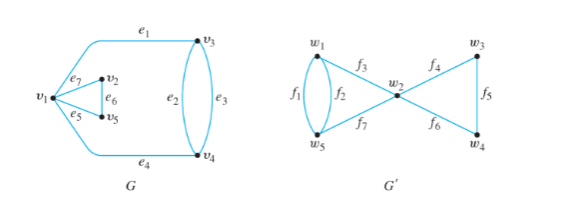
\includegraphics[width=0.6\textwidth]{ figure13.png }
\end{figure}
\pf{Solution}

\noindent To solve this problem, you must find functions g: $V(G) \rightarrow V(G^{\prime})$ and h: $E(G) \rightarrow E(G^{\prime})$ such that for each $v\in V(G)$ and $e \in E(G)$, v is an endpoint of e if, and only if, $g(v)$ is an endpoint of $h(e)$
\bigbreak \noindent
\nt{
	Setting up such functions is partly a matter of trial and error and partly a matter of deduction.
	\vspace{4mm}
	
	For instance, since $e_2$ and $e_3$ are parallel (\textit{have the same endpoint}), $h(e_2)$ and $h(e_3)$ must be parallel also.
}
\bigbreak \noindent
One pair of functions for showing isomorphism between the two graphs is shown below
\newpage
\begin{figure}[ht]
\centering
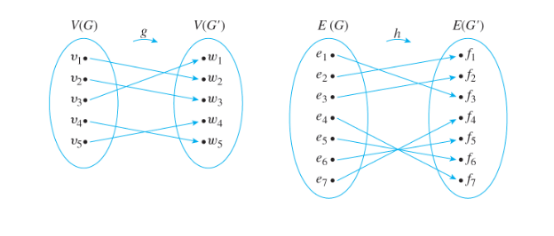
\includegraphics[width=0.7\textwidth]{ figure14.png }
\end{figure}
\bigbreak \noindent 
\begin{large}
	\textbf{\section{Trees}}
\end{large}

\thmcon{
	\textbf{\underline{Definition}}
	\vspace{3mm}

	In mathematics, a tree is a connected graph that does not contain any circuits. Mathematical trees are similar in certain ways to their botanical namesakes.	
	\vspace{3mm}

	A graph is said to be circuit-free if, and only if, it has no circuits. A graph is called a tree if, and only if, it is circuit-free and connected. A \textbf{trivial tree} is a graph that consists of a single vertex. A graph is called a forest if, and only if, it is circuit-free and not connected.
}
\bigbreak \noindent \bigbreak \noindent

\ex{Trees and Non-trees}{
	All the graphs shown in figure {4} are trees, whereas those in figure {5} are not.
}
\bigbreak \noindent 
\begin{figure}[ht]
\centering
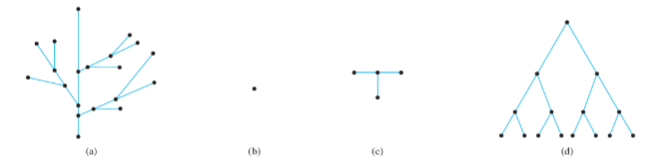
\includegraphics[width=0.6\textwidth]{ figure15.png }
\caption{Trees}
\end{figure}
\bigbreak 
\begin{figure}[ht]
\centering
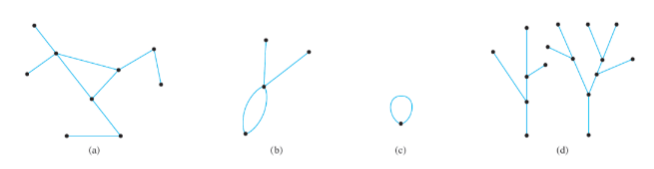
\includegraphics[width=0.55\textwidth]{ figure16.png }
\caption{Non-Trees}
\end{figure}
\pagebreak

\noindent \begin{LARGE}
	\textbf{Examples of Trees}
\end{LARGE}
\bigbreak \noindent \bigbreak \noindent
\ex{A Decision Tree}{
	During orientation week, a college administers a mathematics placement exam to all entering students. The exam consists of two parts, and placement recommendations are made as indicated by the tree shown below in figure 6.
}
\begin{figure}[ht]
\centering
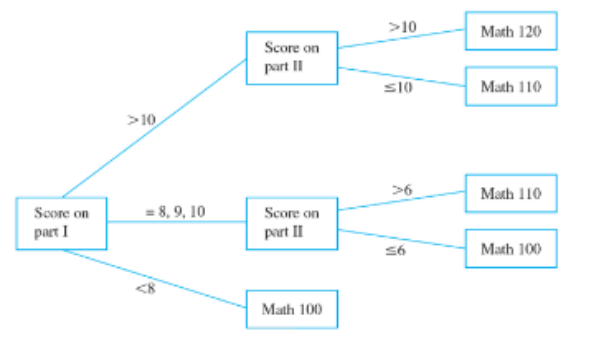
\includegraphics[width=0.6\textwidth]{ figure17.png }
\caption{}
\end{figure}
\bigbreak \noindent
We read the tree from left to right to decide what course should be recommended for a student who scored 9 on part I and 7 on part II.
\vspace{5mm}

Since the student socred 9 on part I, the score on part II is checked.
\vspace{4mm}

Since it is greater than 6, the student should be advised to take Math 110.
\bigbreak \noindent 
\begin{large}
	\textbf{\subsection{Characterizing Trees}} 
\end{large}
\thmcon{
	\textbf{\underline{Defintion}}
	\vspace{3mm}

	There is a somewhat suprising relation between the number of vertices and the number of edges of a tree.
	\vspace{4mm}

	It turns out that if $n$ is a postive integer, then any tree with $n$ vertices (no matter what its shape) has $n-1$ edges.
	\vspace{4mm}

	Perhaps even more surprisingly, a partial converse to this fact is also true - namely, any connected graph with $n$ vertices and $n-1$ edges is a tree.
	\vspace{4mm}

	It follows from these facts that if even one new edge (but no new vertex) is added to a tree, the resulting graph must contain a circuit.
	\vspace{4mm}

	Also, from the fact that removing an edge from a circuit does not disconnect a graph, it can be shown that every connected graph has a subgraph that is a tree.
	\vspace{4mm}

	It follows that if $n$ is a positive integer, any graph with $n$ vertices and \textit{fewer} than $n-1$ edges is not connected.
}
\pagebreak
\thm{}{Any tree that has more than one vertex has at least one vertex of degree 1.}
\bigbreak \noindent
\thm{}{ For any positive integer $n$, any tree with $n$ vertices has $n-1$ edges.}
\bigbreak \noindent 
\thmcon{
	\textbf{\underline{Terminal Vertices}}
	\vspace{3mm}

	Let $T$ be a tree. If $T$ has at least two vertices, then a vertex of degree 1 in $T$ is called a \textbf{leaf} (or a \textbf{terminal vertex}), and a vertex of degree greater than 1 in $T$ is called an \textbf{internal vertex} (or a \textbf{branch vertex}). The unique vertex in a trivial tree is also called a \textbf{leaf} or \textbf{terminal vertex}.
}
\bigbreak \noindent \bigbreak \noindent \bigbreak \noindent
\ex{}{
	Find all leaves (or terminal vertices) and all internal (or branch) vertices in the following tree.
}
\begin{figure}[ht]
\centering
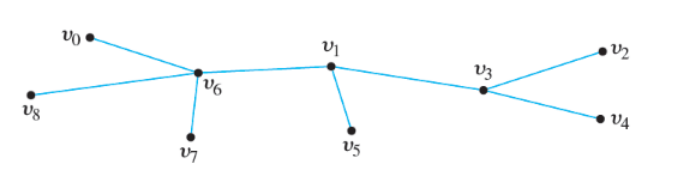
\includegraphics[width=0.64\textwidth]{ tree1.png }
\end{figure}
\pf{Solution}

The terminal vertices are {\large{$$v_0, v_2, v_4, v_5, v_7, v_8$$}}
\vspace{3mm}

The internal vertices are {\large{$$v_6, v_1, v_3$$}}
\bigbreak \noindent \bigbreak \noindent
\vspace{2mm}

\ex{}{
	A graph $G$ has ten vertices and twelve edges. Is it a tree?
}
\pf{Solution}

No, By definition of Theorem 8.2, any tree with ten vertices has nine edges, not twelve.
\pagebreak
\begin{large}
	\textbf{\subsection{Rooted Trees}}
\end{large}
\bigbreak \noindent
\thmcon{
	\textbf{\underline{Defintion}}
	\vspace{3mm}

	In mathematics, a rooted tree is a tree in which one vertex has been distinguished from the others and is designed the \textit{root}. Given any other vertex $v$ in the tree, there is a unique path from the root to $v$.
	\vspace{5mm}

	The number of edges in such a path is called the level of $v$, and the \textit{height} of the tree is the length of the longest such path. It is traditional in drawing rooted trees to place the root at the top and show the branches descending from it.
	\bigbreak \noindent
	A \textbf{rooted tree} is a tree in which there is one vertex that is distinguished from the others and is called the \textbf{root}.
	\vspace{2mm}

	The \textbf{level} of a vertex is the number of edges along the unique path between it and the root. 
	\vspace{2.5mm}

	The \textbf{height} of a rooted tree is the maximum level of any vertex of the tree. Given the root or any internal vertex $v$ of a rooted tree, the \textbf{children} of $v$ are all those vertices that are adjacent to $v$ and are one level farther away from the root than $v$. 
	\vspace{3mm}

	If $w$ is a child of $v$, then $v$ is called the \textbf{parent} of $w$, and two distinct vertices that are both children of the same parent are called \textbf{siblings}. Given two distinct vertices $v$ and $w$, if $v$ lies on the unique path between $w$ and the root, then $v$ is an \textbf{ancestor} of $w$ and $w$ is a \textbf{descendant} of $v$.
}
\bigbreak \noindent
{\centerline{{\large{These terms are illustrated in Figure {7}}}}}
\begin{figure}[ht]
\centering
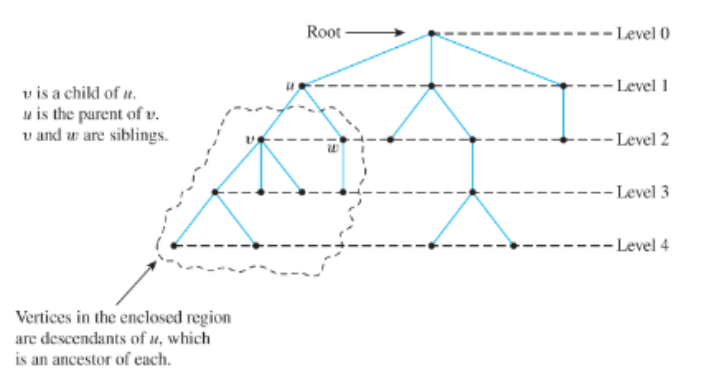
\includegraphics[width=0.7\textwidth]{ rootedtree.png }
\caption{Rooted Tree}
\end{figure}
\ex{}{
	Consider the tree with root $v_0$ shown below.
	\begin{enumerate}
		\begin{multicols}{2}
		\item What is the level of $v_5$? 
		\item What is the level of $v_0$?
		\end{multicols}
		\begin{multicols}{2}
		\item what is the height of this rooted tree?
		\item What are the children of $v_3$
		\end{multicols}
		\begin{multicols}{2}
		\item What is the parent of $v_2$
		\item what are the siblings of $v_8$
		\end{multicols}
		\begin{multicols}{2}
	\item What are the descendants of $v_3$?
	\item How many terminal vertices are on the tree
	\end{multicols}
	\end{enumerate}
}
\pagebreak
\begin{figure}[ht]
\centering
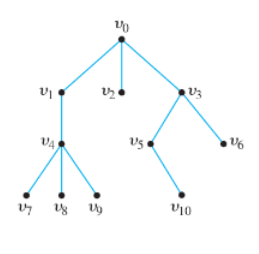
\includegraphics[width=0.4\textwidth]{ tree2.png }
\end{figure}
\pf{Solution}

\begin{center}
	The tree has a level of \textbf{2} since the number of edges from $v_0$ to $v_5$ is $2$. 
	\vspace{2mm}

	The level of $v_0$ is \textbf{0} since there are no edges between $v_0$ and itself.
	\vspace{2mm}
	
	the height of this rooted tree is \textbf{3} since the maximum level of the tree is 3.
	\vspace{2mm}

	The children of $v_3$ are $v_5$ and $v_6$
	\vspace{2mm}

	the parent of $v_2$ is $v_0$
	\vspace{2mm}

	the siblings of $v_8$ are $v_7$ and $v_9$
	\vspace{2mm}

	The descendants of $v_3$ are $v_5$, $v_6$, and $v_10$
	\vspace{2mm}

	There are 6 leaves (terminal vertices) on this rooted tree.
\end{center}
\bigbreak \noindent \bigbreak \noindent
\begin{large}
	\textbf{\subsection{Binary Trees}} 
\end{large}
\thmcon{
	\textbf{\underline{Defintion}}
	\vspace{3mm}

	When every vertex in a rooted tree has at most two children and each child is designated either the (unique) left child or the (unique) right child, the result is a binary tree.
	\vspace{5mm}

	A \textbf{binary tree} is a rooted tree in which every parent has at most two children. 
	\vspace{3mm}

	Each child in a binary tree is designated either a \textbf{left child} or a \textbf{right child} (but not both), and every parent has at most one left child and one right child. 
	\vspace{3mm}

	A \textbf{full binary tree} is a binary tree in which each parent has exactly two children.
	\vspace{3mm}

	Given any parent $v$ in a binary tree $T$, if $v$ has a left child, then the \textbf{left subtree} of $v$ is the binary tree whose root is the left child of $v$, whose vertices consist of the left child of $v$ and all its descendants, and whose edges consist of all those edges of $T$ that connect the vertices of the left subtree. The \textbf{right subtree} of $v$ is defined analogously.
}
\vspace{3mm}

{\centerline{{\large{These terms are illustrated in Figure {8}}}}}
\pagebreak
\begin{figure}[ht]
\centering
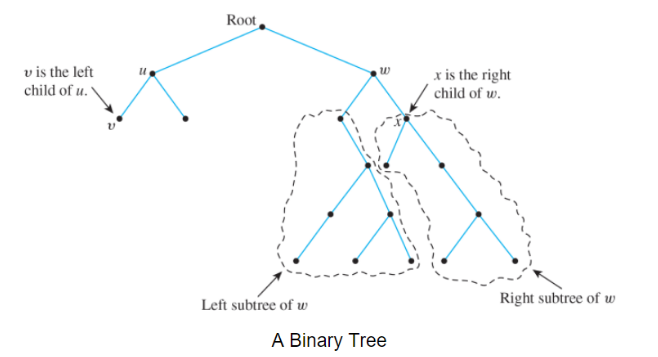
\includegraphics[width=0.6\textwidth]{ binarytree.png }
\caption{A Binary Tree}
\end{figure}
\bigbreak \noindent
An interesting theorem about binary trees says that if you know the number of internal vertices of a full binary tree, then you can calculate both the total number of vertices and the number of leaves, and conversely. More specifically, a full binary tree with $k$ internal vertices has a total of $2 k+1$ vertices of which $k+1$ are leaves.
\bigbreak \noindent
\thm{}{If $k$ is a positive integer and $T$ is a full binary tree with $k$ internal vertices, then (1) $T$ has a total of $2 k+1$ vertices, and (2) $T$ has $k+1$ leaves.}
\bigbreak \noindent \bigbreak \noindent
\ex{Determining Whether a Certain Full binary Tree Exists}{
	Is there a full binary tree that has 10 internal vertices and 13 terminal vertices?
}
\pf{Solution}

No. By Theorem 8.3, a full binary tree with 10 internal vertices has 10 + 1 = 11 leaves, not 13.
\bigbreak \noindent \bigbreak \noindent
\thm{}{
	for every integer $h \ge 0$, if $T$ is any binary tree with height $h$ and $t$ leaves, then
	$$ t \le 2^{h}$$
	Equivalently: $$log_2 t \le h$$
}
\bigbreak \noindent \bigbreak \noindent
\ex{Determining whether a Certain Binary Tree Exists}{
Is there a binary tree that has height 5 and 38 leaves?
}
\pf{Solution}


No. By Theorem 8.4, a binary tree with height 5 and 38 leaves cannot exists because the height is greater 

than $2^5$
\pagebreak
\nt{A full binary tree of height $h$ has $2^h$ leaves.}
\bigbreak \noindent \bigbreak \noindent
\begin{large}
	\textbf{\subsection{Binary Search Trees}} 
\end{large}
\bigbreak \noindent
\thmcon{
	\textbf{\underline{Defintion}}
	\vspace{3mm}

	A binary search tree is a kind of binary tree in which data records, such as customer information, can be stored, searched, and processed very efficiently. To place records into a binary search tree, it must be possible to arrange them in a total order.
	\vspace{4mm}

	In case they do not have a natural total order of their own, an element of a totally ordered set, such as a number or a word and called a \textbf{key}, may be added to each record. The keys are inserted into the vertices of the tree and provide access to the records to which they are attached.
	\vspace{5mm}

	Once it is built, a binary search tree has the following property: 
	\vspace{2mm}

	for every internal vertex $v$, all the keys in the \textbf{left subtree} of $v$ are \textbf{less} than the key in $v$, and all the keys in the \textbf{right subtree} of $v$ are \textbf{greater} than the key in $v$.
	\vspace{5mm}

For example, check that the following is a binary search tree for the set of records with the following keys: $$15,10,19,25,12,4$$
}
\begin{figure}[ht]
\centering
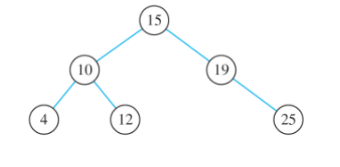
\includegraphics[width=0.5\textwidth]{ tree3.png }
\caption{Binary Search Tree for the data listed above}
\end{figure}
\begin{mdframed}
 \begin{large}
	 \vspace{2mm}

  To build a binary search tree, start by making a root and insert a key into it.
  \vspace{5mm}

\noindent To add a new key, compare it to the key at the root. If the new key is less than the key at the root, give the root a left child and insert the new key into it.
\vspace{4mm}

\noindent If the key is greater than the key at the root, give the root a right child and insert the new key into it.
\vspace{4mm}

\noindent So to add a key at a subsequent stage, work down the tree to find a place to put the new key, starting at the root and either moving left or right depending on whether the new key is less or greater than the key at the vertex to which it is currently being compared.t
 \end{large} 

\end{mdframed}
\pagebreak
\begin{figure}[ht]
  \centering
  \subfigure{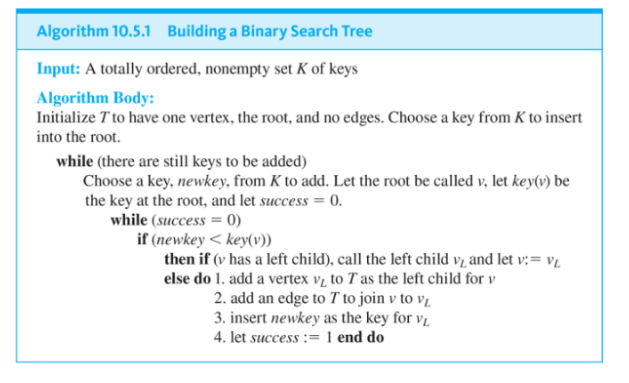
\includegraphics[width=0.7\textwidth]{tree4.png}}
  \hfill
  \subfigure{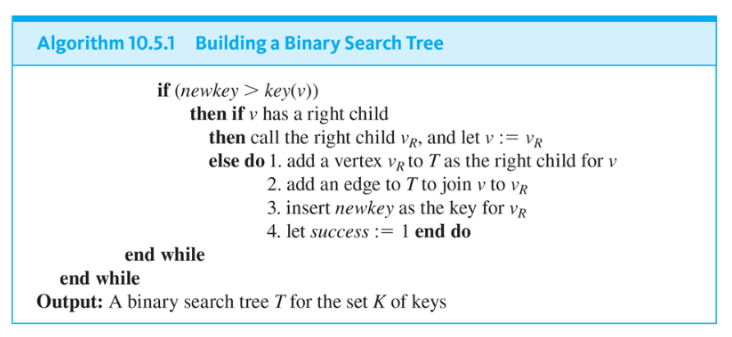
\includegraphics[width=0.7\textwidth]{tree5.png}}
  \caption{Binary search tree algorithm}
\end{figure}
\bigbreak \noindent \bigbreak \noindent
\ex{Building a Binary search tree}{
	Go through the steps to build a binary search tree for the keys $15,10,19,25,12,4$, and insert the keys in the order in which they are listed. For simplicity, use the same names for the vertices and their associated keys.
}
\pf{Solution}

\textbf{Insert 15}: Make 15 the root.
\vspace{3mm}

\textbf{Insert 10}: Compare 10 to 15.
\vspace{3mm}

Since $10<15$ and 15 does not have a left child, make 10 the left child of 15 and add an edge joining 15 

and 10.
\vspace{3mm}

\textbf{Insert 19}: Compare 19 to 15.
\vspace{3mm}

Since $19>15$ and 15 does not have a right child, make 19 the right child of 15 and add an edge joining 15 

and 19.
\vspace{3mm}

\textbf{Insert 25}: Compare 25 to 15.
\vspace{3mm}

Since $25>15$ and 15 has a right child, namely 19, 
\vspace{3mm}

compare 25 to 19.
\vspace{3mm}

Since $25>19$ and 19 does not have a right child, make 25 the right child of 19 and add an edge joining 19 

and 25.
\vspace{3mm}

\textbf{Insert 12}: Compare 12 to 15.
Since $12<15$ and 15 has a left child, namely 10, 
\vspace{3mm}

compare 12 to 10 .
Since $12>10$ and 10 does not have a right child, make 12 the right child of 10 and add 

an edge joining 10 and 12.
\vspace{3mm}

\textbf{Insert 4}: Compare 4 to 15.
\vspace{3mm}

Since $4<15$ and 15 has a left child, namely 10,
\vspace{3mm}

compare 4 to 10.
\vspace{3mm}

Since $4<10$ and 10 does not have a left child, make 4 the left child of 10 and add an edge joining 10 and 

4.
\bigbreak \noindent
\vspace{1.5mm}

{\centerline{{\large{\textbf{The sequence of steps is shown in the following diagrams}}}}}
\begin{figure}[ht]
\centering
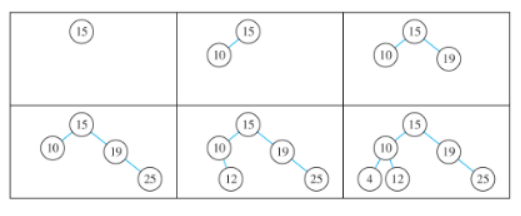
\includegraphics[width=0.5\textwidth]{ tree6.png }
\caption{Steps for building the example tree}
\end{figure}
\bigbreak \noindent \bigbreak \noindent
\begin{large}
	\textbf{\subsection{Spanning Trees}}
\end{large}






\end{document}


